\documentclass{beamer}

\usefonttheme{serif}

\setbeamertemplate{footline}[frame number]{}
\setbeamertemplate{navigation symbols}{}

\usecolortheme{default}
\setbeamercolor{block title}{bg=lily!20,fg=black}
\setbeamercolor{block body}{bg = blue!10, fg = black}
\setbeamertemplate{itemize item}[square]
\setbeamercolor{itemize item}{fg = cyan}
\setbeamercolor{enumerate item}{fg = cyan}

\usetheme{default}

%\setbeamercolor{titlelike}{fg=cyan}
%Information to be included in the title page:
\title{Sample title}
\author{Anonymous}
\institute{Overleaf}
\date{2021}

\title[About Beamer] %optional
{Helium–Neon Laser}

%\subtitle{A short story}

\author[Arthur, Doe] % (optional, for multiple authors)
{A.~Simankovich \and D.~Dedkov }

\institute[VFU] % (optional)
{
	Moscow Institute of Physics and Technology
}

\date[VLC 2023] % (optional)
%{Very Large Conference, April 2021}

%\logo{\includegraphics[height=1cm]{overleaf-logo}}

\begin{document}
	
	\frame{\titlepage}
	
	\begin{frame}
		\frametitle{Abstract}
		TODO

	\end{frame}
	
	\begin{frame}
		\frametitle{Elementary processes}
		
		\begin{columns}[t]
			\footnotesize
			
			\column{0.33\linewidth}
			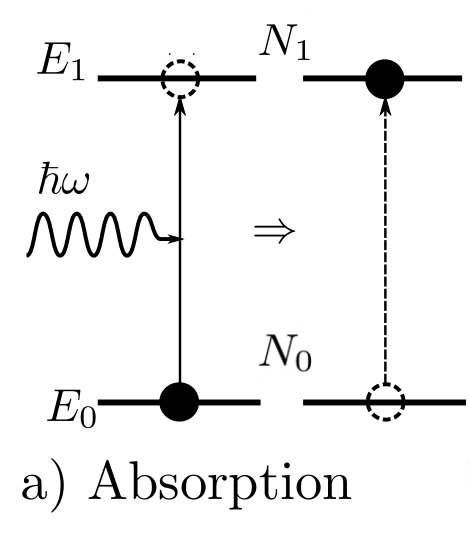
\includegraphics[height=3cm]{res/emission_types_1.jpg}
			$$\left(\frac{dN_0}{dt}\right)_{\text{abs}} = - B_{01} N_0 \rho(\omega)$$
			Einstein coefficients are the same $B_{01} = B_{10} = B$ 

			\column{0.33\linewidth}
			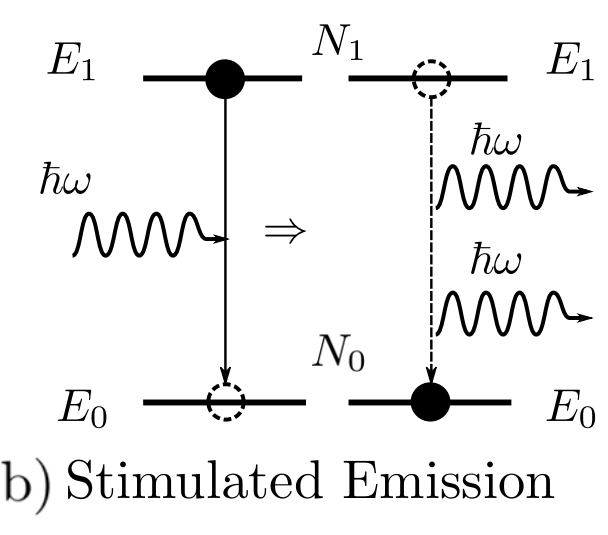
\includegraphics[height=3cm]{res/emission_types_2.jpg}
			$$\left(\frac{dN_0}{dt}\right)_{\text{stim}} = B_{10} N_1 \rho(\omega)$$
			phase, direction and frequency of emitted and external photons are identical.
		
			\column{0.33\linewidth}
			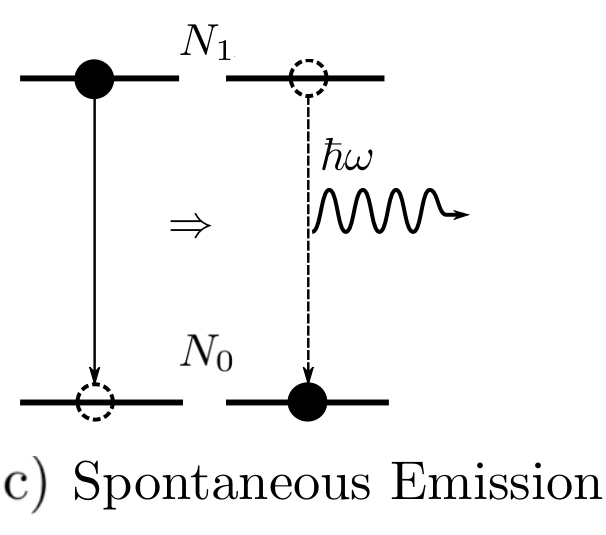
\includegraphics[height=3cm]{res/emission_types_3.jpg}
			$$\left(\frac{dN_0}{dt}\right)_{\text{spon}} = - A_{10} N_1$$
			photons radiate independently in all directions. $\frac{dN_0}{dt}$ \textbf{does not} depend on $\rho(\omega)$.
		
		\end{columns}
		\vspace{10pt}
		\footnotesize
		Where $\rho(\omega)$ -- spectral energy density of the isotropic radiation field at the frequency of the transition.
	\end{frame}

	\begin{frame}
	\frametitle{Laser Gain}
	
	\begin{figure}
		\centering
		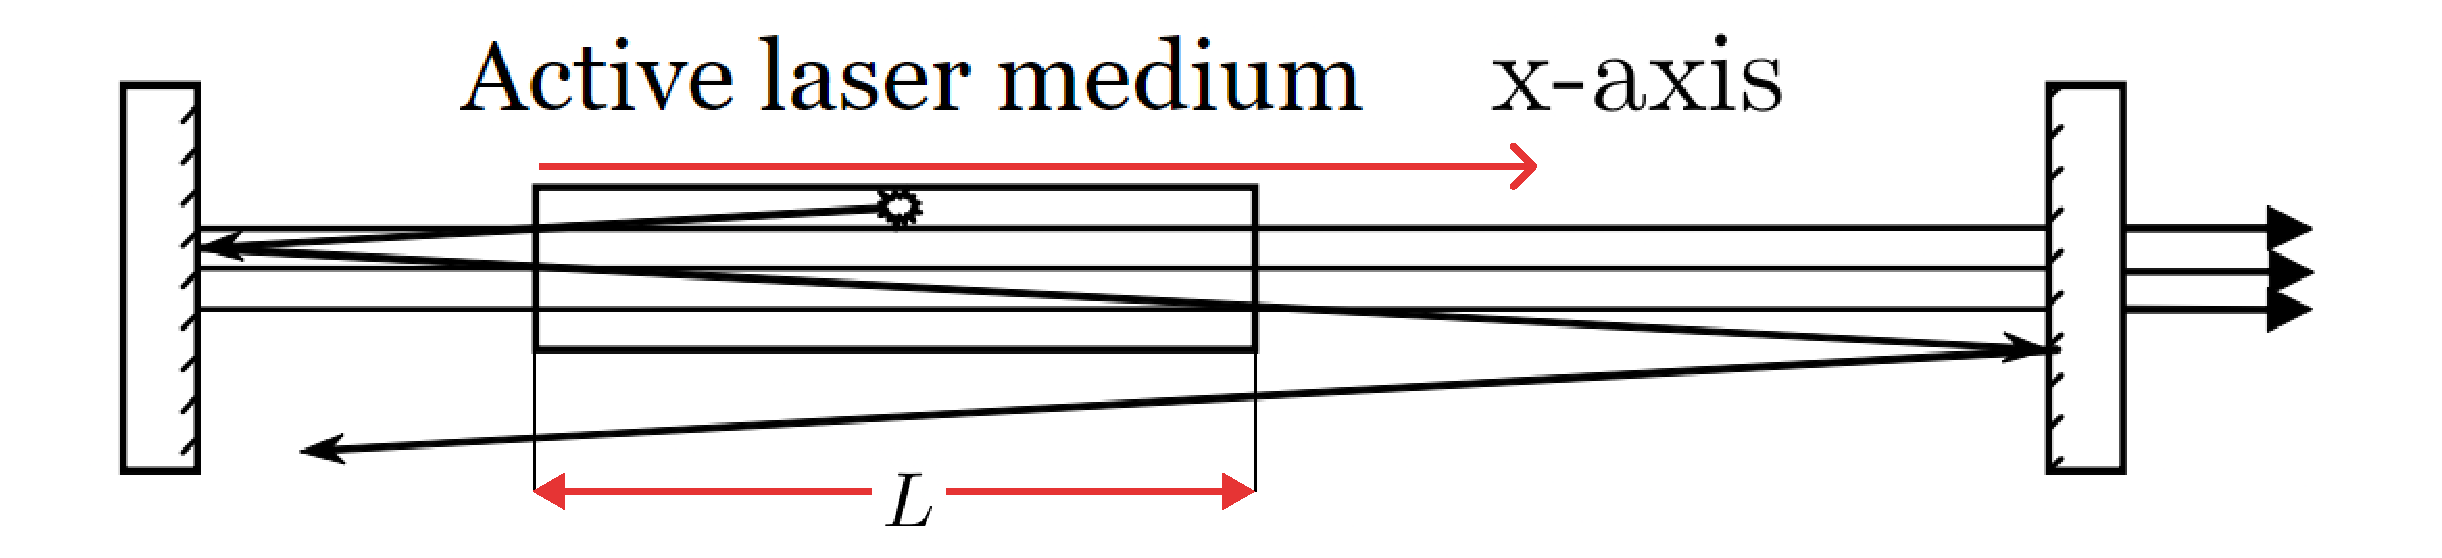
\includegraphics[width=1\linewidth]{res/general_laser_scheme.pdf}
		\caption{General laser scheme}
		\label{fig:general_laser_scheme}
	\end{figure}
	Beer–Lambert–Bouguer law states that intensity of light $I(x)$ changes:
	$$I(x) = I_0 \exp({\gamma x}),$$
	
	where $\gamma$ -- medium gain coefficient. With length $L$ gain per period is called \textbf{laser gain}:
	
	$$G = \exp{(2\gamma L)}.$$
	\end{frame}
	
	\begin{frame}
		\frametitle{Population inversion}
		The fact that the number of spontaneously emitted photons does not depend on  $\rho(\omega)$ gives us a reason to neglect $\left(\frac{dN_0}{dt}\right)_{\text{spon}}$ term. Number of photons emitted at a time $dt$:
		
		\begin{equation} \label{eq1}
			\begin{split}
				\frac{dN}{dt} & = \left(\frac{dN_0}{dt}\right)_{\text{abs}} + \left(\frac{dN_0}{dt}\right)_{\text{stim}} =  B (N_1 - N_0) \rho(\omega)
			\end{split}
		\end{equation}

		Therefore:
		\begin{equation}
			\gamma = \frac{dI}{I} = \frac{dN \cdot \hbar\omega}{\rho(\omega)} = B\frac{\hbar\omega }{v} (N_1 - N_0), 
		\end{equation}
		where $v = \frac{c}{n}$ -- speed of light inside medium.
		
		\vspace*{20px}
		\centering
		$\gamma$ is positive if $N_1 > N_0$. This laser principle is called \textbf{population inversion}
	\end{frame}

	\begin{frame}
		\frametitle{Generation spectrum}
		
		\begin{columns}
			\column{0.6\linewidth}
			\begin{figure}
				\centering
				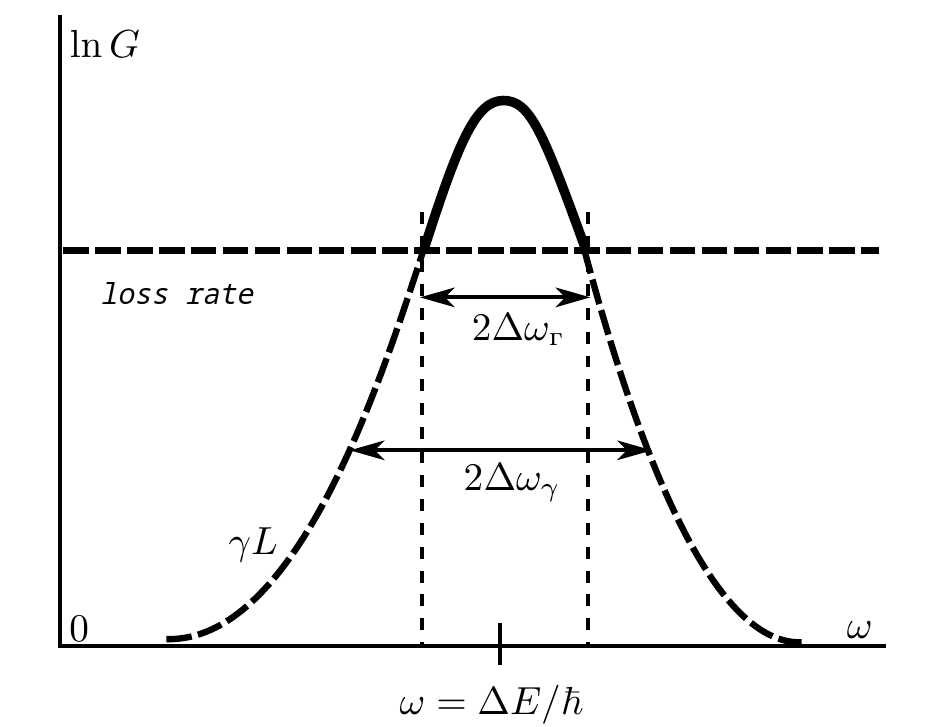
\includegraphics[width=1\linewidth]{res/generation_spectrum.png}
			\end{figure}
			\column{0.4\linewidth}
			Generation spectrum of He-Ne laser is defined by three factors: natural broadening, Doppler broadening and loss rate.
			$$ \omega_n \approx 2 \pi / \tau_n \Rightarrow \nu_n \approx10^{8} \text{ Hz} , $$
			$\tau_n \approx 10^{-8} \text{ s}$ -- lifetime of $630$ nm  $Ne$ transition.
		\end{columns}
				
		$$ \omega_D \approx \omega \frac{v_T}{c}, \approx 1.5 \cdot 10^9 \text{ Hz}$$
		$v_T$ -- thermal motion velocity (assuming $T = 400$ K).
		
		And loss rate reduces spectrum even further:
		$$ 2 \gamma L > - \ln{K} - \ln{r_1 r_2}, $$
		$r_1, r_2$ -- mirrors reflectance, $K$ -- part of remaining intensity.
	\end{frame}
	

	\begin{frame}
		\frametitle{Longitudinal Modes}
		Mode -- stationary wave pattern in resonator with particular frequency and spatial distribution.
		
		\begin{figure}
			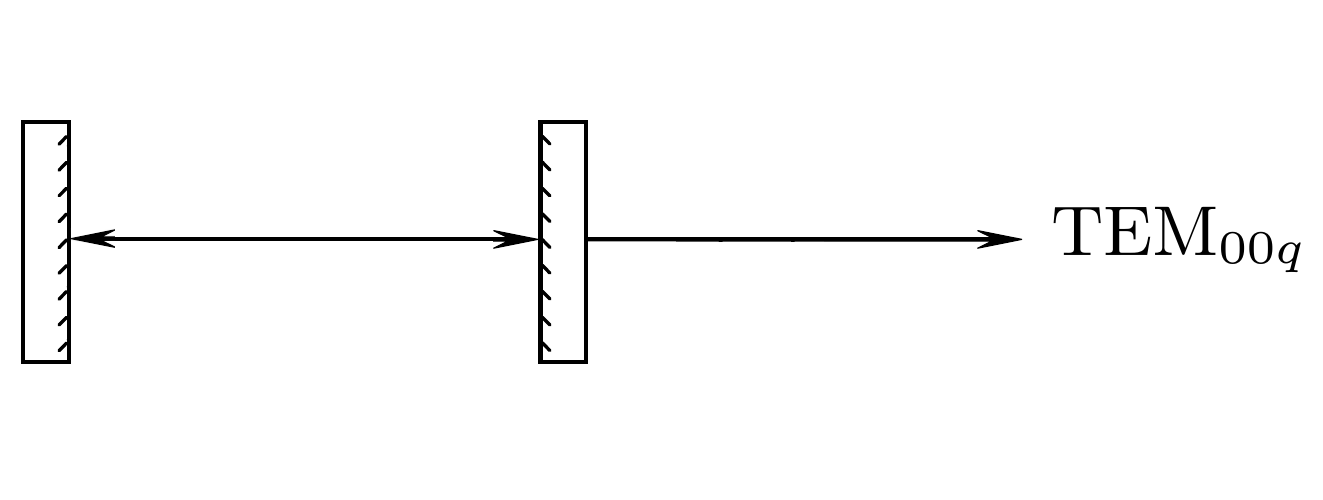
\includegraphics[width=0.5\linewidth]{res/tem00q.png}
			\caption{Longitudinal modes}
		\end{figure}
		
		Most of the energy in resonator cavity is concentrated in standing waves. Therefore, condition on $TEM_{00q}$ modes goes as follows:
		
		$$ L = q \frac{\lambda}{2} \; \Rightarrow \; \omega_q = q \frac{\pi c}{L} \approx 2 \pi \cdot 150 \text{ MHz}, \; q \in \mathcal{N},$$
		$L \approx 1$ m.
	\end{frame}
	
	\begin{frame}
		\frametitle{Modes spectrum}
		
		Every $TEM_{00q}$ gives narrow spectrum $\omega_q \pm \Delta \Omega_{TEM}$.
		\begin{figure}
			\centering
			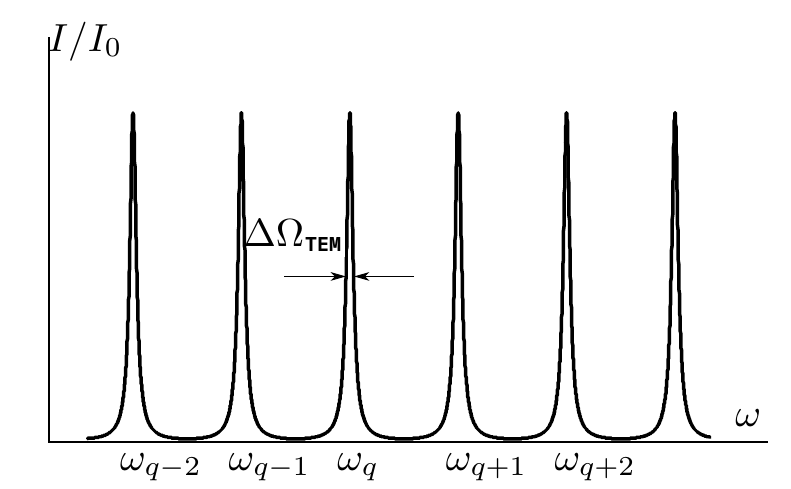
\includegraphics[width=0.5\linewidth]{res/tem_spectrum.png}
		\end{figure}
		
		Taking into account that
		$$\Delta \Omega_{TEM} \approx \frac{\omega_q}{Q},$$
		$Q$ -- Q-factor, and using common parameters of He-Ne laser we get:
		$$ \Omega_{TEM} \approx 2 \pi \cdot 10^6 \text{ Hz}.$$
		
	\end{frame}
	
	\begin{frame}
		\frametitle{Singlemode and multimode}
		
		Applying modes spectrum to generation spectrum we get:
		
		\begin{figure}
			\centering
			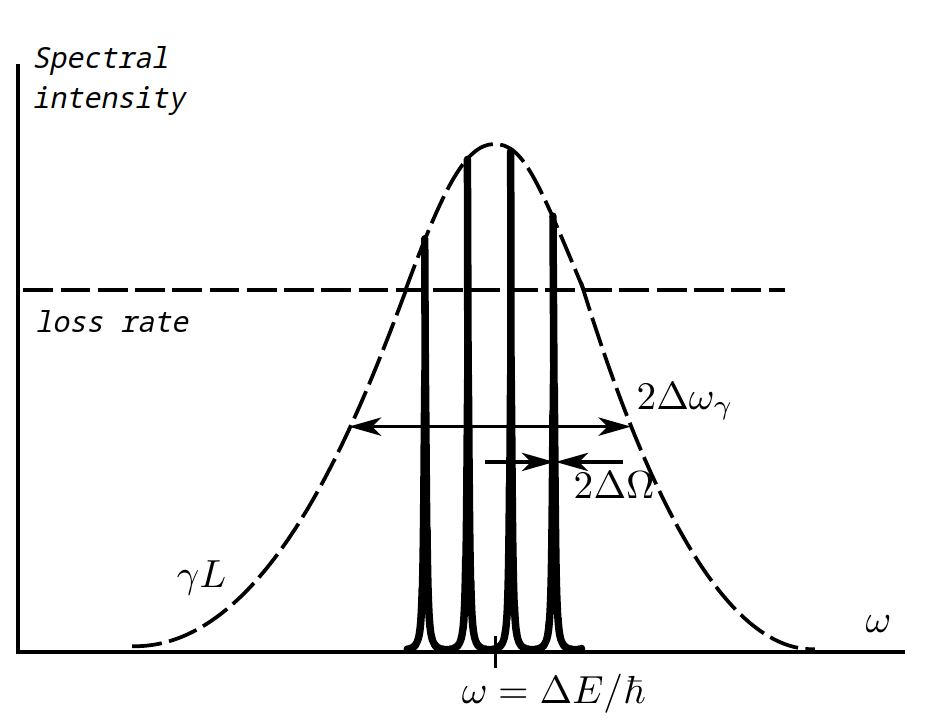
\includegraphics[width=0.6\linewidth]{res/overall_spectrum.png}
		\end{figure}
	
		In generation spectrum, created by medium, resonator spectrum cuts off a few frequencies.
		
		Estimating maximal number of modes:
		$$ N_m = \omega_D / \omega_n \approx 10.$$
	\end{frame}

	\begin{frame}
		\frametitle{Polarization of Laser Emission}
		\begin{figure}
			\centering
			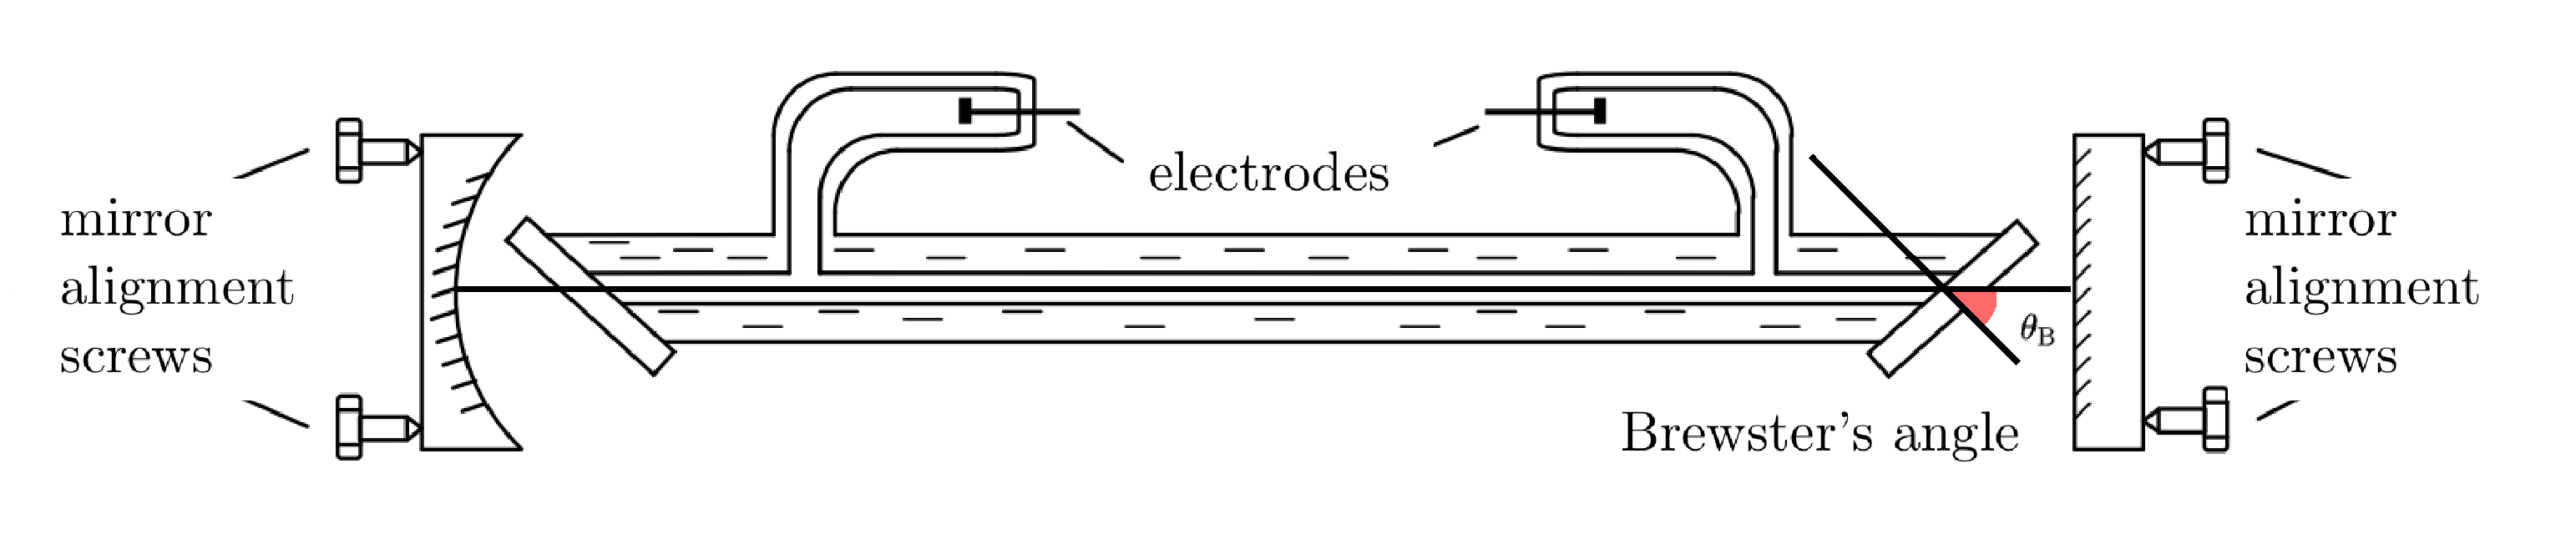
\includegraphics[width=1\linewidth]{res/brewster_setup.pdf}
		\end{figure}
		
		\begin{columns}
			\begin{column}{0.3\textwidth}
				\begin{figure}
					\centering
					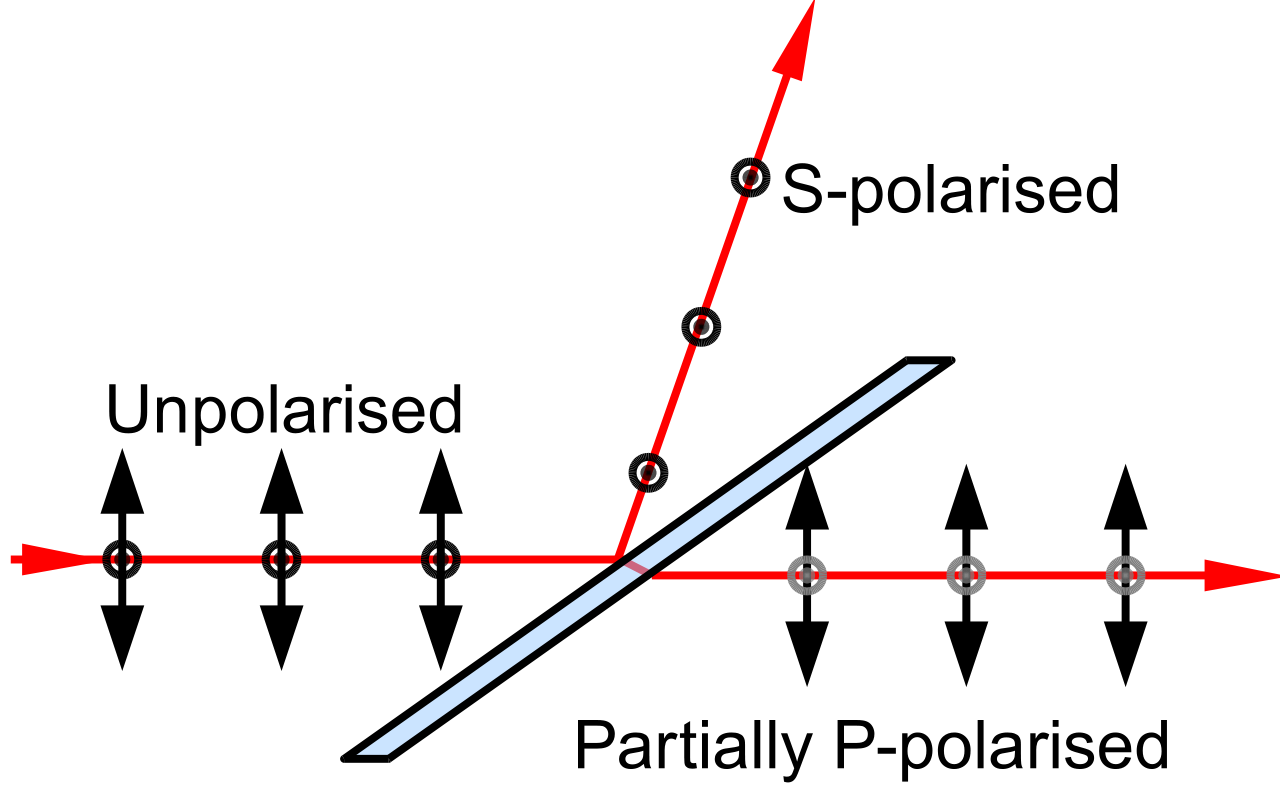
\includegraphics[width=1\linewidth]{res/brewsters-angle.svg}
				\end{figure}
			\end{column}
			\begin{column}{0.7\textwidth}
				To remove reflections from laser's windows the Brewster's angle properties can be used:
				$$r_p = \frac{E_r}{E_i} = \frac{n_2 \cos{\theta_i} - n_1 \cos{\theta_t}}{n_2 \cos{\theta_i} + n_1 \cos{\theta_t}}\bigg\rvert_{\theta_i = \theta_B} = 0$$
			\end{column}
		\end{columns}	
	\end{frame}
	
	\begin{frame}
		\frametitle{Malus' law}
		\begin{columns}
		\begin{column}{0.4\textwidth}
			\begin{figure}
				\centering
				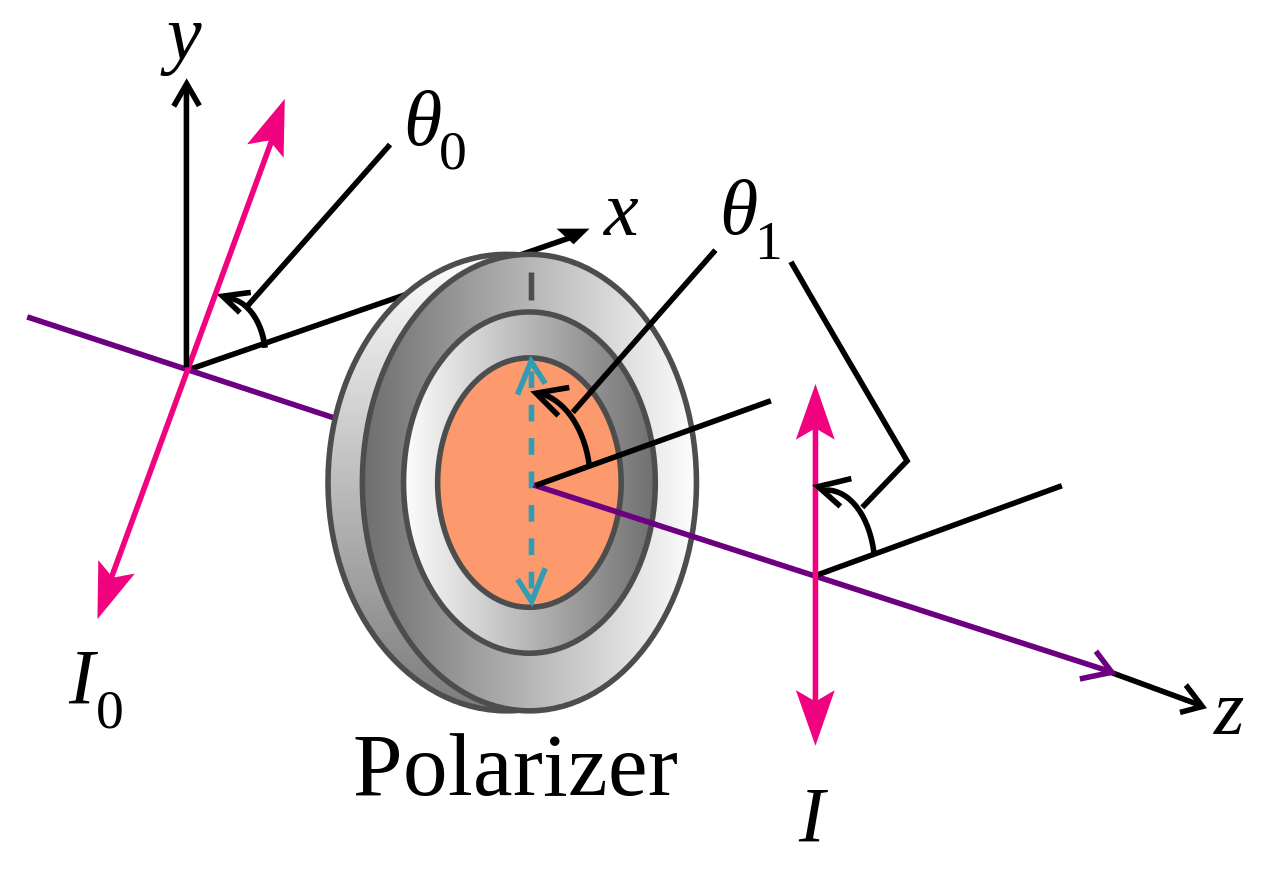
\includegraphics[width=1\linewidth]{res/malus_law.png}
				\caption{Malus' law (here $\theta_i = \theta_1 - \theta_0$)}
			\end{figure}
		\end{column}
		\begin{column}{0.6\textwidth}
			 To study the laser's polarization, polaroid and Malus' law is used:
			 \begin{equation}
				 I(\theta_i) = I_0 \cos^2{\theta_i},
				 \label{eq:malus}
			 \end{equation}
			 
			 where $I_0$ is the initial intensity and $\theta_i$ is the angle between the light's initial polarization direction and the axis of the polarizer.
			 
		\end{column}
		\end{columns}	
	\end{frame}


	\begin{frame}[plain,c]
		
		\begin{center}
			\huge \usebeamercolor[fg]{frametitle} Measurements and Results
		\end{center}
		
	\end{frame}
	
	
	\begin{frame}
		\frametitle{Experimental setup}
		\begin{figure}
			\centering
			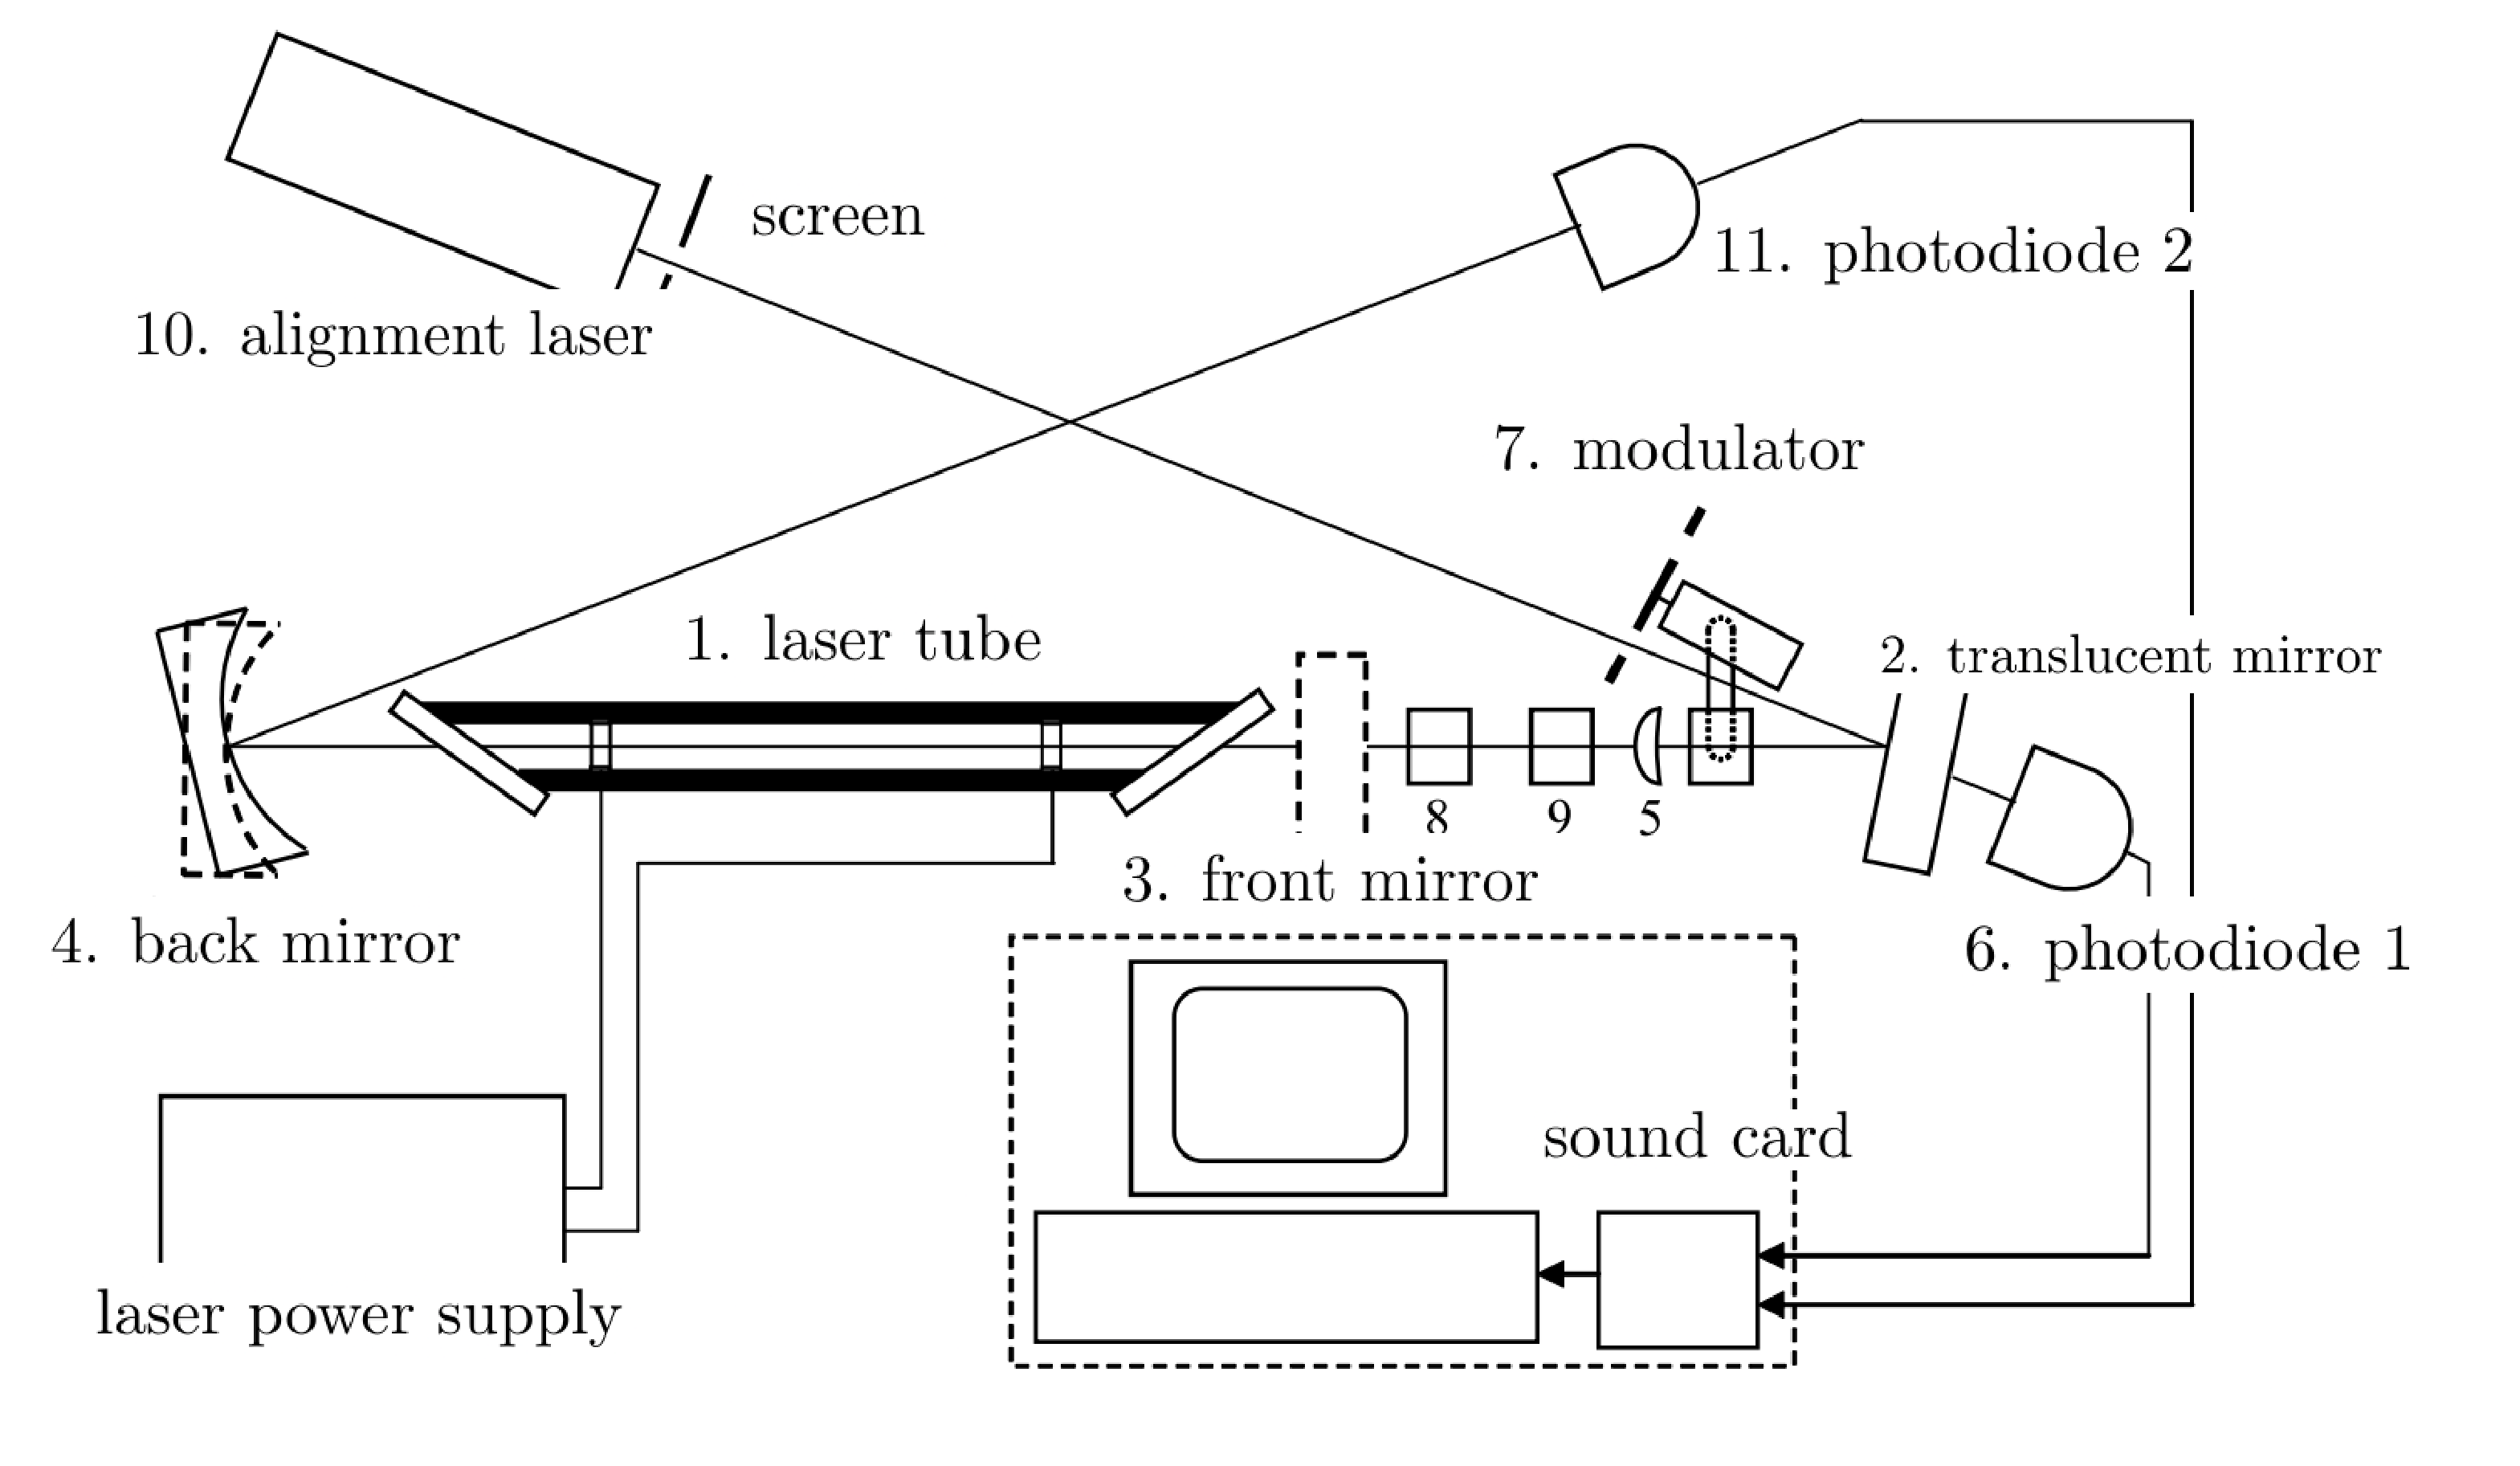
\includegraphics[width=1.1\linewidth]{res/experimental_setup.pdf}
		\end{figure}
		
	\end{frame}
	
	
	\begin{frame}
		\frametitle{Experimental Setup}
	
		\begin{figure}
			\centering
			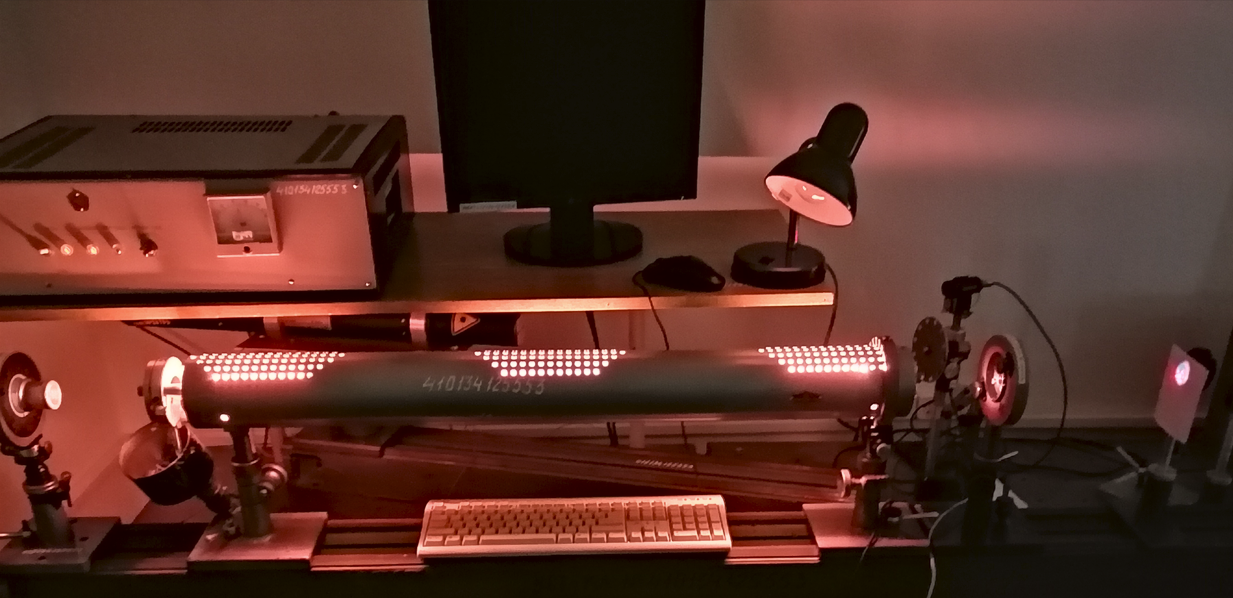
\includegraphics[width=1\linewidth]{res/setup.png}
			\caption{Photo of laboratory setup}
		\end{figure}
	\end{frame}
	
	\begin{frame}
		\frametitle{Adjustment}
		\begin{columns}
			\column{0.5\linewidth}
			\begin{figure}
				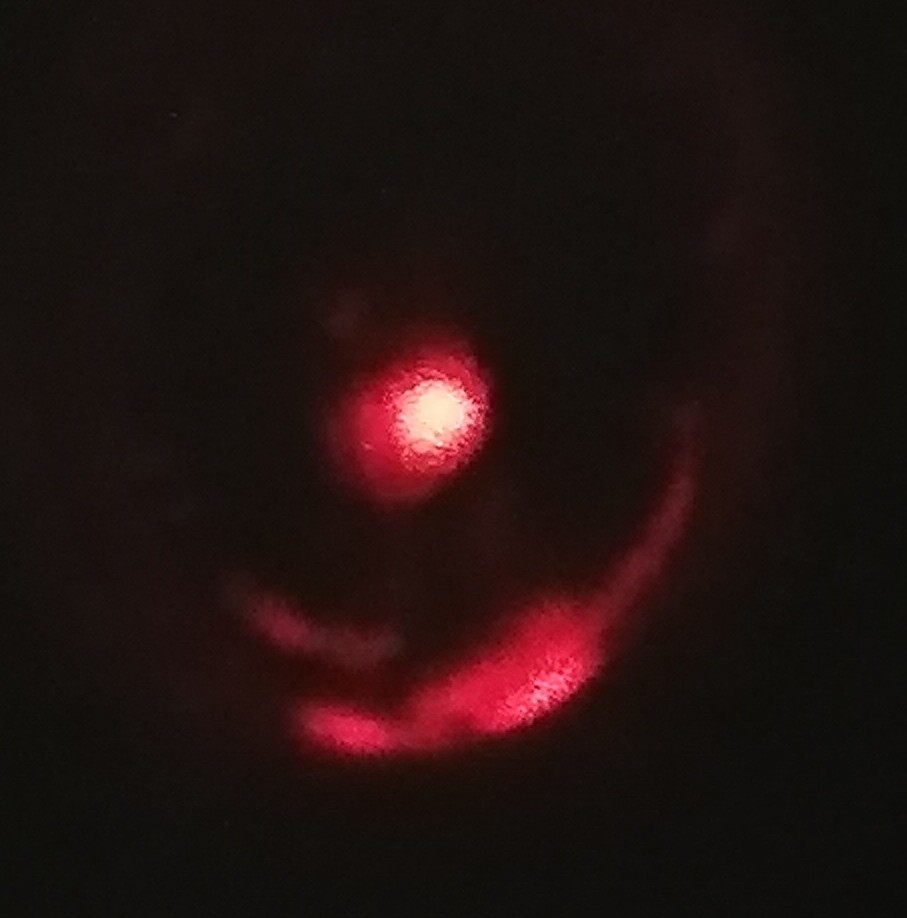
\includegraphics[width=4cm]{data/beam.jpg}
				\caption{Image of laser beam after laser tube}
			\end{figure}
			\column{0.5\linewidth}
			Laser gain is measured with additional laser and a pair of photodiodes. We need laser beam to pass through laser tube without dissipation on tube walls.
		\end{columns}
		
		To achieve laser generation we need fine adjustment of front and back mirrors of laser. Additional laser is used for that purpose. We adjust back mirror until reflection of alignment laser appears over it's output window. The same procedure applies to the front mirror.
	\end{frame}
	
	
	\begin{frame}
		\frametitle{Laser Gain}
		Laser gain is measured using two photodiodes, connected to sound card. To exclude the influence of photodiodes dark current and ambient illumination we use modulator. Therefore, we can measure AC. Intensities are measured with and without amplification ($I_i^{\text{on}}$ and $I_i^{\text{off}}$).
		
		\begin{columns}
			\begin{column}{0.4\textwidth}
				\begin{figure}
					\centering
					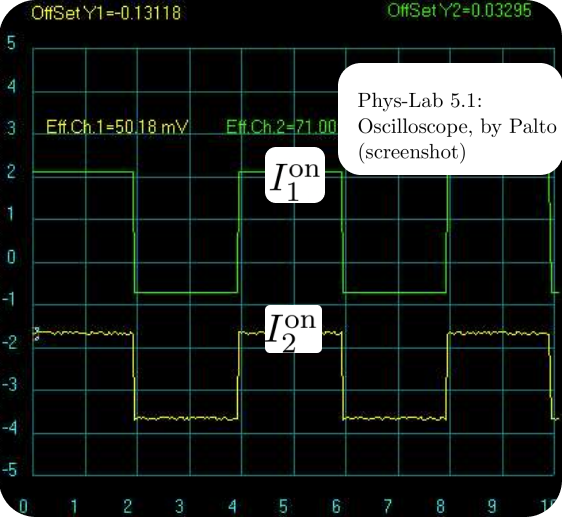
\includegraphics[width=1\linewidth]{res/oscilloscope.png}
					\caption{Phys-Lab 5.1: Oscilloscope, by Palto (screenshot)}
				\end{figure}
			\end{column}
			\begin{column}{0.6\textwidth}
				Photodiodes are connected to the sound card with the ADC. This gives us a direct way to measure intensity. 
				
				$$G = \left(\frac{I^{\text{on}}_{1}}{I^{\text{off}}_{1}}\right)/\left(\frac{I^{\text{on}}_{2}}{I^{\text{off}}_{2}}\right),$$
				
				where $I_i^j$ -- r.m.s. light intensity.
				
				Series of measurments gives the following result:
				$$G = 1.029 \pm 0.006$$
			\end{column}
		\end{columns}
		
	\end{frame}
		
	
	\begin{frame}
		\frametitle{Laser Polarization}
		When laser generation is active we can measure polarization. Polarization is measured using single photodiode and normalized.
		\vspace{-20pt}
		\begin{columns}
			\begin{column}{0.6\textwidth}
				\begin{figure}
					\centering
					\includegraphics[width=1.1\linewidth]{gen/cosine.pdf}
					\caption{Intensity for different polaroid angles}
				\end{figure}
			\end{column}
			\begin{column}{0.4\textwidth}
				Interpolating according to (\ref{eq:malus}):
				$$I(\theta) = A \cos^2{(\Omega \theta + \theta_0)},$$
				We obtain the following parameters' values: 
				
				\begin{itemize}
					\item[] $\Omega = 0.998 \pm 0.005$
					\item[] $\theta_0 = (-70 \pm 1)^\circ$
				\end{itemize}
			
			This demonstrates that Malus's law holds with a great precision.
			\end{column}
		\end{columns}
		
		
	\end{frame}
	
	
	
	\begin{frame}
		\frametitle{Gain}
		The fact that the number of spontaneously emitted photons does not depend on  $\rho(\omega)$ gives us a reason to neglect $\left(\frac{dN_0}{dt}\right)_{\text{spon}}$ term. Number of 
		
		1. laser tube
		
		laser power supply
		
		4. back mirror
		
		3. front mirror
		
		sound card
		
		2. translucent mirror
		
		6. photodiode 1
		
		11. photodiode 2
		
		7. modulator
		
		screen
		
		10. alignment laser
		Brewster's angle
	
	
	
	\end{frame}
	
\end{document}